\documentclass{article}

\makeatletter
\def\input@path{{Formatting_Instructions_For_NeurIPS_2026/}}
\makeatother
\usepackage[preprint]{neurips_2026}
\usepackage[utf8]{inputenc}
\usepackage[T1]{fontenc}
\usepackage{hyperref}
\usepackage{url}
\usepackage{booktabs}
\usepackage{amsfonts}
\usepackage{nicefrac}
\usepackage{microtype}
\usepackage{xcolor}
\usepackage{graphicx}
\usepackage{amsmath}

\title{HW2: Transfer Learning for Flowers102 Classification}

\author{%
  Student Report\\
  Deep Learning and Spatial Intelligence\\
}

\begin{document}

\maketitle

\begin{abstract}
This report presents four experiments on Flowers102 image classification: ImageNet-pretrained ResNet fine-tuning, hyperparameter analysis, pretraining ablation, and attention/Transformer comparison. The baseline ResNet-18 and ResNet-34 models reached 89.85\% and 89.64\% test accuracy, respectively. Hyperparameter tuning improved the best ResNet result to 91.59\% test accuracy with ResNet-34 using classifier learning rate $5\times10^{-4}$ and backbone learning rate $5\times10^{-5}$. The pretraining ablation showed the largest effect: ResNet-18 dropped from 89.85\% to 28.41\% test accuracy when trained from scratch, and ResNet-34 dropped from 89.64\% to 21.01\%. In the final comparison, Swin-T achieved the best overall result with 94.51\% best validation accuracy and 92.24\% test accuracy.
\end{abstract}
% 中文注释：摘要直接按四个任务概括实验，并引用真实结果数值。

\section{Dataset and Common Setup}

The experiments use the 102 Category Flower Dataset through \texttt{torchvision.datasets.Flowers102} \citep{nilsback2008flowers}. The official split contains 1020 training images, 1020 validation images, and 6149 test images over 102 classes. This means that each class has only a small number of labeled training examples, so the task is a good setting for studying transfer learning.
% 中文注释：这里简要说明 Flowers102 的官方划分和小样本特点。

For training images, I use \texttt{RandomResizedCrop(224)}, \texttt{RandomHorizontalFlip}, \texttt{ColorJitter}, \texttt{ToTensor}, and ImageNet normalization. For validation and test images, I use \texttt{Resize(256)}, \texttt{CenterCrop(224)}, \texttt{ToTensor}, and the same ImageNet normalization. All reported runs use top-1 accuracy as the main metric. The optimizer is AdamW with weight decay $1\times10^{-4}$, random seed 42, and the MPS device on a local Mac.
% 中文注释：这里说明统一的数据增强、归一化、优化器和评价指标。

\section{Task 1: ImageNet-pretrained ResNet Baseline}

\subsection{Method}

For the first task, I fine-tune ResNet-18 and ResNet-34 \citep{he2016resnet}. Both models are initialized with ImageNet-pretrained weights \citep{deng2009imagenet}. I replace the original 1000-way fully connected layer with a new 102-way classifier for Flowers102. The pretrained backbone and the new classifier use different learning rates: the backbone learning rate is $1\times10^{-4}$, while the classifier learning rate is $1\times10^{-3}$. This design lets the ImageNet features change slowly while allowing the randomly initialized classifier to adapt quickly.
% 中文注释：Task 1 的做法是加载 ImageNet 预训练 ResNet，替换最后分类层，并使用分层学习率微调。

\subsection{Results}

Table~\ref{tab:task1} shows the baseline results. ResNet-18 reached 92.16\% best validation accuracy and 89.85\% test accuracy. ResNet-34 reached 91.76\% best validation accuracy and 89.64\% test accuracy. In this baseline setting, the deeper ResNet-34 did not outperform ResNet-18; the two models are very close, with ResNet-18 slightly higher by 0.21 percentage points on the test split.
% 中文注释：Task 1 结果显示 ResNet-18 和 ResNet-34 的 baseline 表现接近，ResNet-18 略高。

\begin{table}[t]
  \caption{Task 1 baseline fine-tuning results. Accuracies are percentages.}
  \label{tab:task1}
  \centering
  \small
  \resizebox{\linewidth}{!}{%
\begin{tabular}{llrrrrrrr}
\toprule
Folder & Model & Pretrained & Epochs & BS & Backbone LR & Classifier LR & Best Val & Test \\
\midrule
task1\_resnet18 & resnet18 & True & 30 & 32 & 1e-4 & 1e-3 & 92.16 & 89.85 \\
task1\_resnet34 & resnet34 & True & 30 & 32 & 1e-4 & 1e-3 & 91.76 & 89.64 \\
\bottomrule
\end{tabular}
}%

\end{table}

The ResNet-18 training curve in Figure~\ref{fig:task1_curve} shows fast improvement in the first few epochs. The best validation checkpoint appears before the last epoch, so saving the best validation model is important for this dataset.
% 中文注释：这里结合训练曲线说明 best checkpoint 的必要性。

\begin{figure}[t]
  \centering
  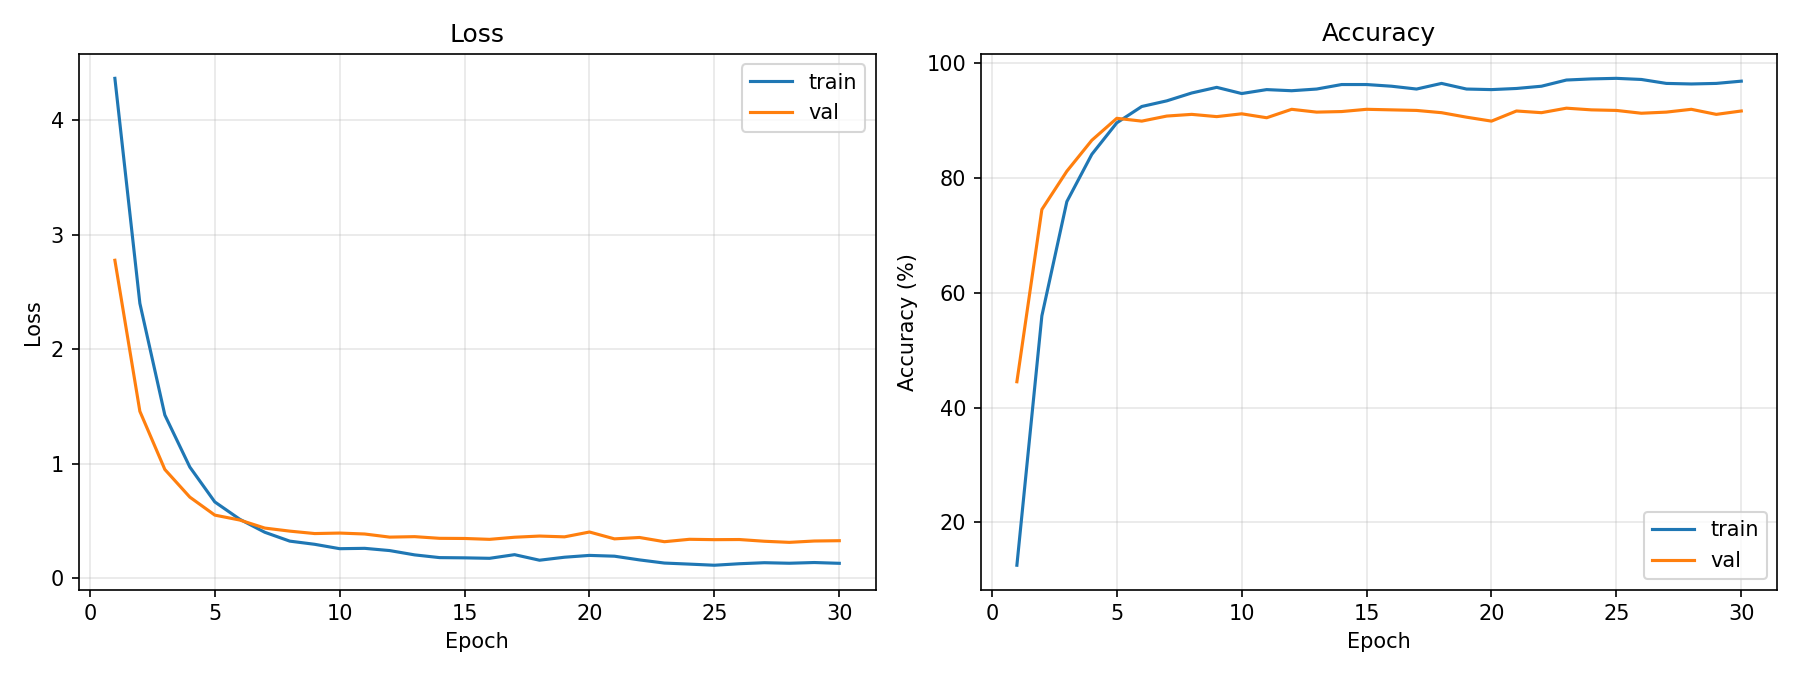
\includegraphics[width=\linewidth]{figures/task1_resnet18_curve.png}
  \caption{Task 1 ResNet-18 baseline training and validation curves.}
  \label{fig:task1_curve}
\end{figure}

\section{Task 2: Hyperparameter Analysis}

\subsection{Method}

For Task 2, I keep ImageNet-pretrained ResNet-18 and ResNet-34, but manually change epoch count, classifier learning rate, backbone learning rate, and batch size. The classifier learning rate is treated as the main learning rate, while the backbone learning rate is set to one tenth of it. The tested classifier learning rates are $1\times10^{-4}$, $5\times10^{-4}$, $1\times10^{-3}$, and $2\times10^{-3}$. I also compare 10, 30, and 50 training epochs, and batch sizes 16 and 32.
% 中文注释：Task 2 的做法是手动改变训练轮数、学习率和 batch size，并保持 backbone 学习率为 classifier 的 0.1 倍。

\subsection{Results for ResNet-18}

Table~\ref{tab:task2_18} gives the ResNet-18 hyperparameter results. The best ResNet-18 setting is 30 epochs, batch size 32, backbone learning rate $5\times10^{-5}$, and classifier learning rate $5\times10^{-4}$, which reaches 94.12\% best validation accuracy and 90.62\% test accuracy. Compared with the Task 1 baseline test accuracy of 89.85\%, this is a 0.77 point improvement.
% 中文注释：ResNet-18 的最佳超参数组合是 classifier lr 5e-4 和 backbone lr 5e-5。

\begin{table}[t]
  \caption{Task 2 hyperparameter analysis for ResNet-18.}
  \label{tab:task2_18}
  \centering
  \small
  \begin{tabular}{rrrrrr}
\toprule
Epochs & BS & Backbone LR & Classifier LR & Best Val & Test \\
\midrule
10 & 32 & 1e-4 & 1e-3 & 91.18 & 89.19 \\
30 & 16 & 1e-4 & 1e-3 & 91.76 & 87.40 \\
30 & 32 & 1e-5 & 1e-4 & 89.22 & 85.59 \\
30 & 32 & 5e-5 & 5e-4 & 94.12 & 90.62 \\
30 & 32 & 1e-4 & 1e-3 & 92.16 & 89.85 \\
30 & 32 & 2e-4 & 2e-3 & 89.31 & 85.64 \\
50 & 32 & 1e-4 & 1e-3 & 92.25 & 89.74 \\
\bottomrule
\end{tabular}

\end{table}

The learning rate comparison is the clearest part of the result. With classifier learning rate $1\times10^{-4}$, ResNet-18 only reaches 85.59\% test accuracy, which suggests slow adaptation. With classifier learning rate $2\times10^{-3}$, test accuracy is 85.64\%, suggesting the update is too aggressive. The moderate $5\times10^{-4}$ setting performs best. Training for 50 epochs does not improve test accuracy over 30 epochs under the standard $1\times10^{-3}$ classifier learning rate, and reducing batch size from 32 to 16 lowers test accuracy from 89.85\% to 87.40\%.
% 中文注释：这里分析 ResNet-18 中学习率过小、过大、训练更久和 batch size 改变的影响。

\begin{figure}[t]
  \centering
  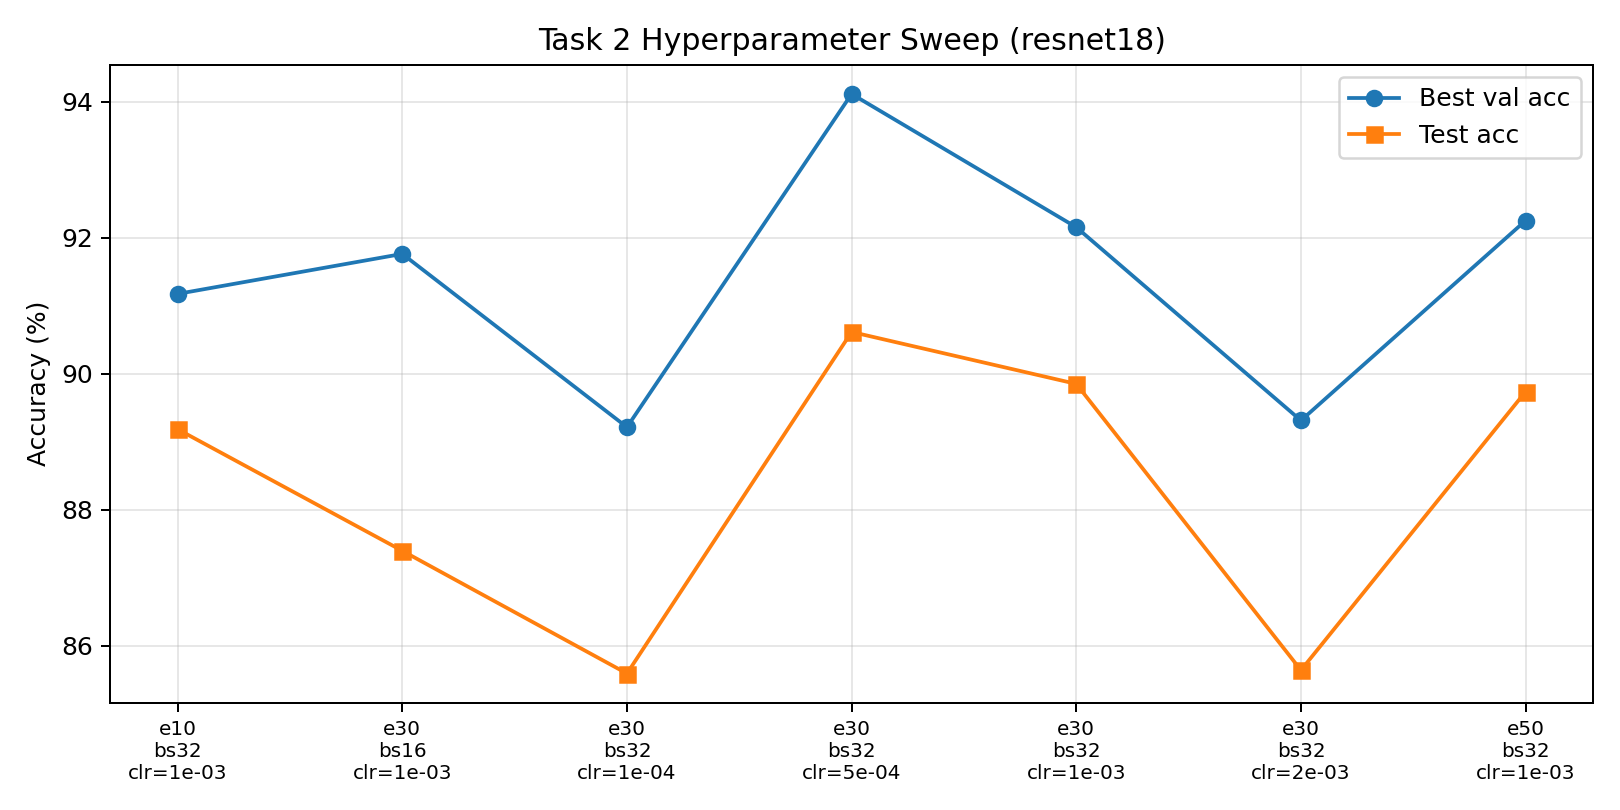
\includegraphics[width=\linewidth]{figures/task2_resnet18_hparam.png}
  \caption{Task 2 ResNet-18 hyperparameter sweep. Each tick shows epochs, batch size, and classifier learning rate.}
  \label{fig:task2_18}
\end{figure}

\subsection{Results for ResNet-34}

Table~\ref{tab:task2_34} gives the ResNet-34 hyperparameter results. The best ResNet-34 setting is also classifier learning rate $5\times10^{-4}$ and backbone learning rate $5\times10^{-5}$, reaching 93.53\% best validation accuracy and 91.59\% test accuracy. This is the best ResNet-only result in the whole experiment.
% 中文注释：ResNet-34 的最佳超参数组合与 ResNet-18 一致，并取得最佳 ResNet 结果。

\begin{table}[t]
  \caption{Task 2 hyperparameter analysis for ResNet-34.}
  \label{tab:task2_34}
  \centering
  \small
  \begin{tabular}{rrrrrr}
\toprule
Epochs & BS & Backbone LR & Classifier LR & Best Val & Test \\
\midrule
10 & 32 & 1e-4 & 1e-3 & 91.76 & 89.64 \\
30 & 16 & 1e-4 & 1e-3 & 91.18 & 88.78 \\
30 & 32 & 1e-5 & 1e-4 & 90.98 & 88.06 \\
30 & 32 & 5e-5 & 5e-4 & 93.53 & 91.59 \\
30 & 32 & 1e-4 & 1e-3 & 91.76 & 89.64 \\
30 & 32 & 2e-4 & 2e-3 & 87.84 & 85.85 \\
50 & 32 & 1e-4 & 1e-3 & 91.76 & 89.64 \\
\bottomrule
\end{tabular}

\end{table}

The same pattern appears for ResNet-34: $1\times10^{-4}$ is too small and gives 88.06\% test accuracy, while $2\times10^{-3}$ is too large and gives 85.85\%. The tuned $5\times10^{-4}$ setting is clearly better than the original $1\times10^{-3}$ baseline. Under the original learning rate, increasing epochs from 30 to 50 does not improve the test result, and the batch size 16 run is lower than batch size 32. These results suggest that learning rate tuning matters more than simply training longer.
% 中文注释：这里分析 ResNet-34 的超参数趋势，说明合适学习率比盲目增加 epoch 更重要。

\begin{figure}[t]
  \centering
  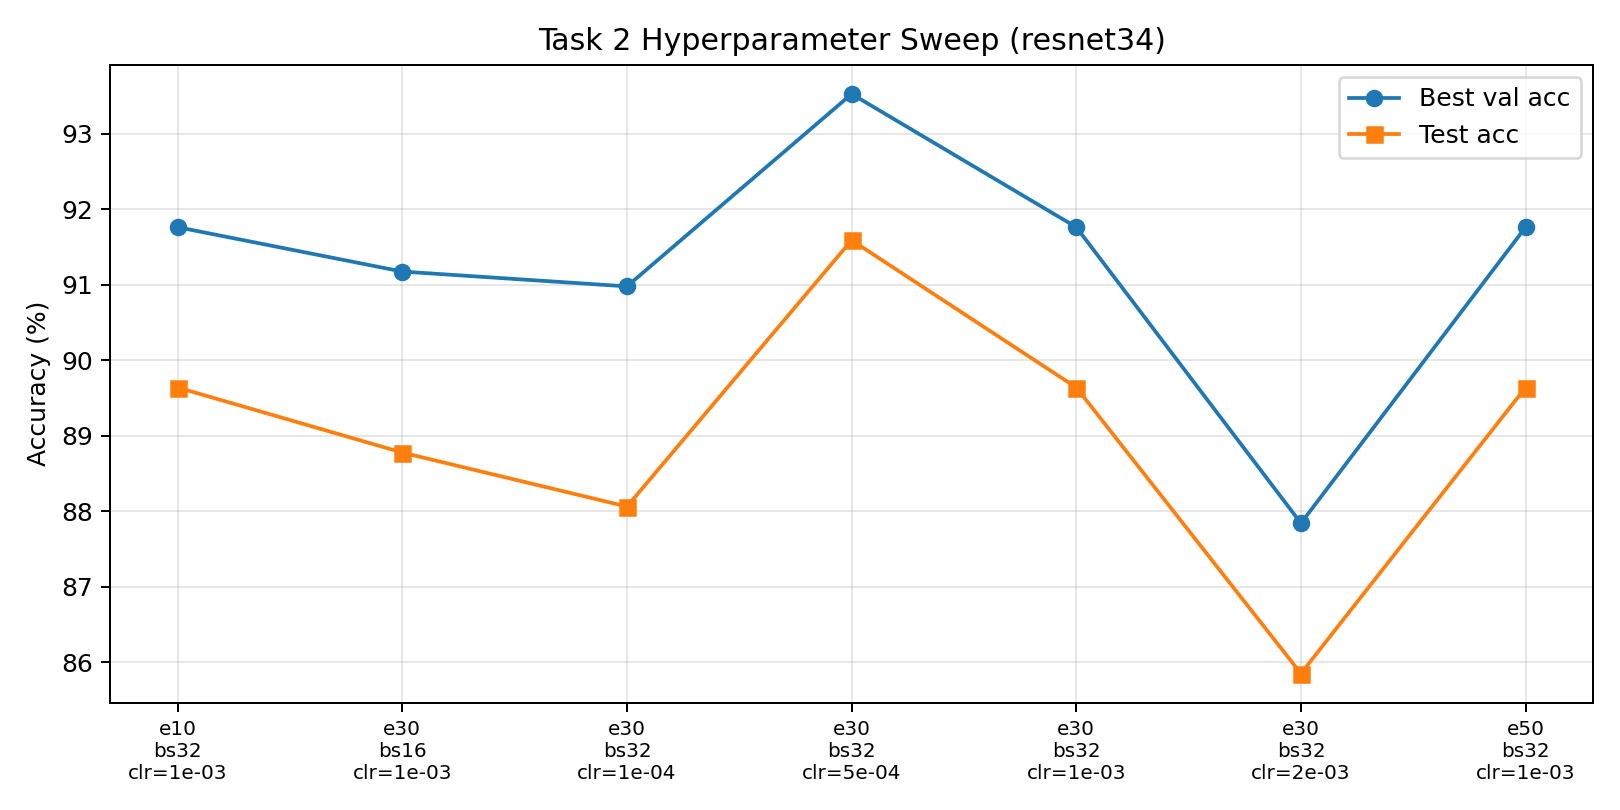
\includegraphics[width=\linewidth]{figures/task2_resnet34_hparam.png}
  \caption{Task 2 ResNet-34 hyperparameter sweep. The $5\times10^{-4}$ classifier learning rate gives the best ResNet-only test accuracy.}
  \label{fig:task2_34}
\end{figure}

\section{Task 3: Pretraining Ablation}

\subsection{Method}

For Task 3, I compare ImageNet-pretrained initialization with random initialization. The network architecture is still ResNet-18 or ResNet-34, and the output layer is changed to 102 classes. The pretrained runs use backbone learning rate $1\times10^{-4}$ and classifier learning rate $1\times10^{-3}$. The scratch runs use learning rate $1\times10^{-3}$ for both backbone and classifier, since all parameters must be learned from the Flowers102 training set.
% 中文注释：Task 3 的做法是比较 ImageNet 预训练和随机初始化，其他训练设置尽量保持一致。

\subsection{Results}

Table~\ref{tab:task3} shows that pretraining is the most important factor in the project. ResNet-18 improves from 28.41\% test accuracy when trained from scratch to 89.85\% with ImageNet pretraining, a gain of 61.44 percentage points. ResNet-34 improves from 21.01\% to 89.64\%, a gain of 68.63 percentage points.
% 中文注释：Task 3 结果显示预训练带来了 61 到 69 个百分点的巨大提升。

\begin{table}[t]
  \caption{Task 3 pretraining ablation.}
  \label{tab:task3}
  \centering
  \small
  \begin{tabular}{llrr}
\toprule
Model & Initialization & Best Val & Test \\
\midrule
resnet18 & pretrained & 92.16 & 89.85 \\
resnet18 & scratch & 32.16 & 28.41 \\
resnet34 & pretrained & 91.76 & 89.64 \\
resnet34 & scratch & 25.98 & 21.01 \\
\bottomrule
\end{tabular}

\end{table}

The curves in Figure~\ref{fig:task3_curves} make this difference visible. The pretrained ResNet-18 quickly reaches high validation accuracy, while the scratch model remains around 30\% validation accuracy after 30 epochs. This supports the conclusion that Flowers102 is too small for training these ResNets from random initialization within the current training budget.
% 中文注释：曲线进一步说明从零训练难以在小训练集上学到足够好的表示。

\begin{figure}[t]
  \centering
  \begin{minipage}{0.49\linewidth}
    \centering
    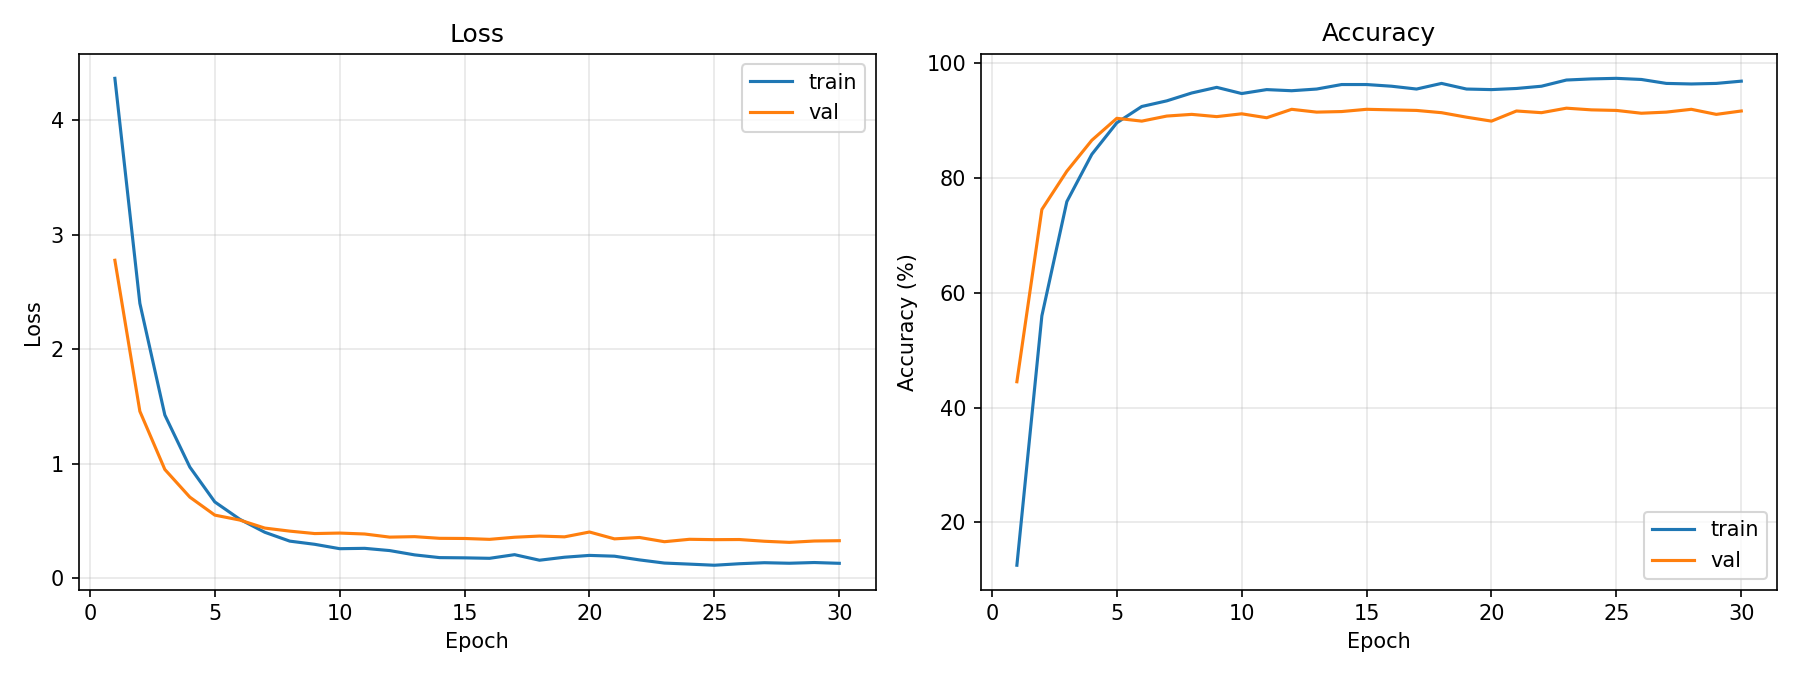
\includegraphics[width=\linewidth]{figures/task3_resnet18_pretrained_curve.png}
    \centerline{\small Pretrained}
  \end{minipage}
  \begin{minipage}{0.49\linewidth}
    \centering
    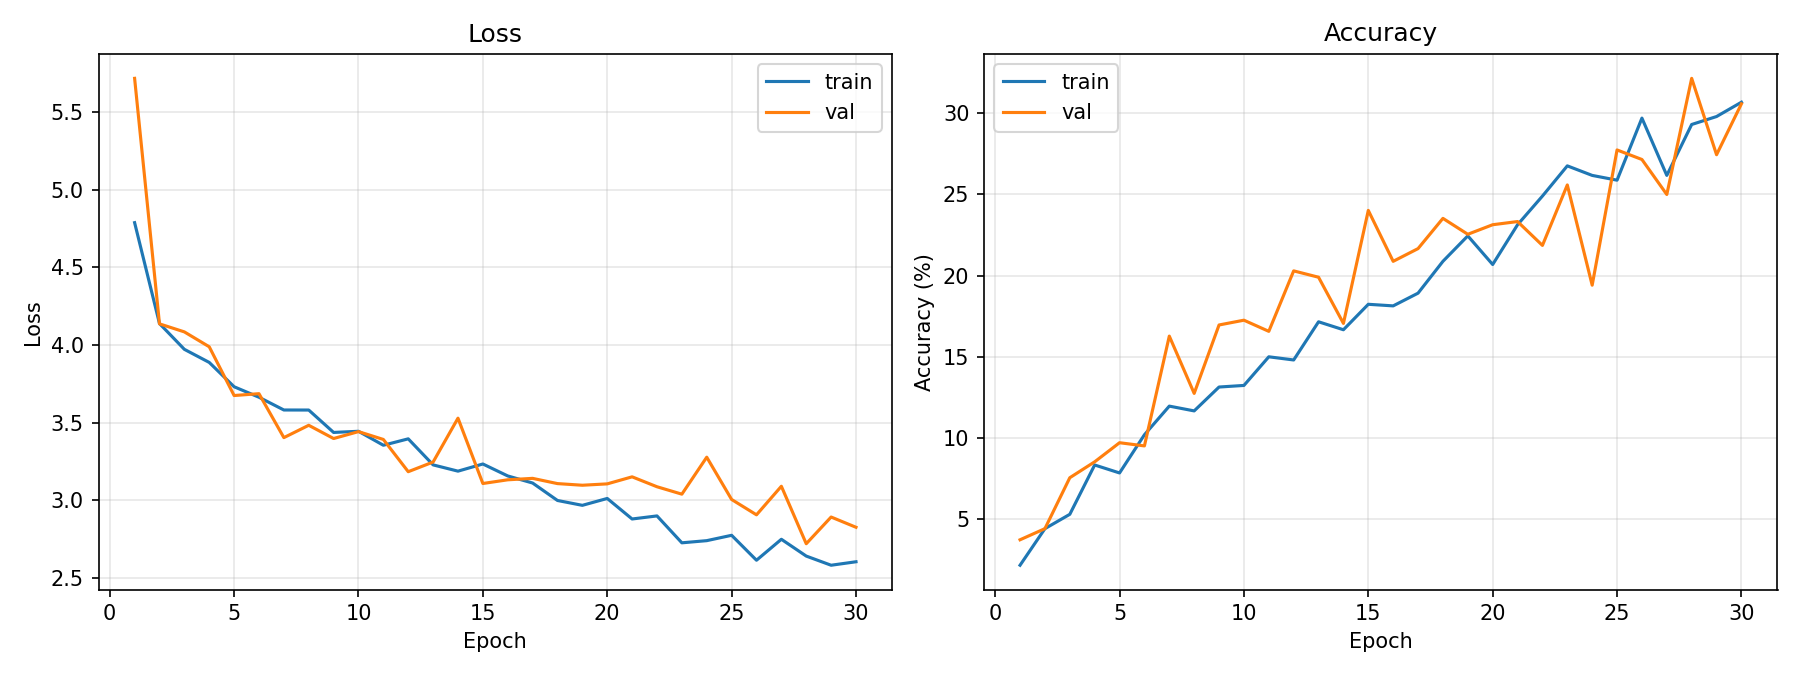
\includegraphics[width=\linewidth]{figures/task3_resnet18_scratch_curve.png}
    \centerline{\small Scratch}
  \end{minipage}
  \caption{Task 3 ResNet-18 pretraining ablation curves.}
  \label{fig:task3_curves}
\end{figure}

\section{Task 4: Attention Mechanisms and Transformer Models}

\subsection{Method}

For Task 4, I test two directions. First, I manually add SE-block and CBAM to the ResNet BasicBlock. SE-block applies channel-wise attention using global pooling and a small gating network \citep{hu2018senet}. CBAM applies both channel attention and spatial attention \citep{woo2018cbam}. The attention ResNets reuse matching ResNet pretrained weights when possible, while the new attention modules are randomly initialized.
% 中文注释：Task 4 的第一部分是在 ResNet block 中手动加入 SE 和 CBAM 注意力模块。

Second, I compare two lightweight Transformer models: ViT-Tiny and Swin-T \citep{dosovitskiy2021vit,liu2021swin}. Both are initialized with pretrained weights and use a 102-class output head. ViT-Tiny uses batch size 8 and learning rate $1\times10^{-4}$, while the recorded Swin-T run uses batch size 32 and learning rate $1\times10^{-4}$.
% 中文注释：Task 4 的第二部分是比较 ViT-Tiny 和 Swin-T 两种轻量 Transformer 架构。

\subsection{Results}

Table~\ref{tab:task4} summarizes the attention and Transformer results. In these runs, SE and CBAM do not improve over the plain ResNet baselines. For ResNet-18, SE reaches 87.87\% test accuracy and CBAM reaches 81.36\%, both below the 89.85\% baseline. For ResNet-34, SE reaches 87.23\% and CBAM reaches 83.77\%, both below the 89.64\% baseline.
% 中文注释：Task 4 中 SE 和 CBAM 在当前训练设置下没有超过普通 ResNet baseline。

\begin{table}[t]
  \caption{Task 4 attention and Transformer comparison.}
  \label{tab:task4}
  \centering
  \small
  \begin{tabular}{lllrr}
\toprule
Model & Attention / Architecture & Pretrained & Best Val & Test \\
\midrule
resnet18 & se & True & 90.78 & 87.87 \\
resnet18 & cbam & True & 85.29 & 81.36 \\
resnet34 & se & True & 90.20 & 87.23 \\
resnet34 & cbam & True & 88.24 & 83.77 \\
vit\_tiny & vit\_tiny & True & 91.27 & 87.58 \\
swin\_t & swin\_t & True & 94.51 & 92.24 \\
\bottomrule
\end{tabular}

\end{table}

\begin{figure}[t]
  \centering
  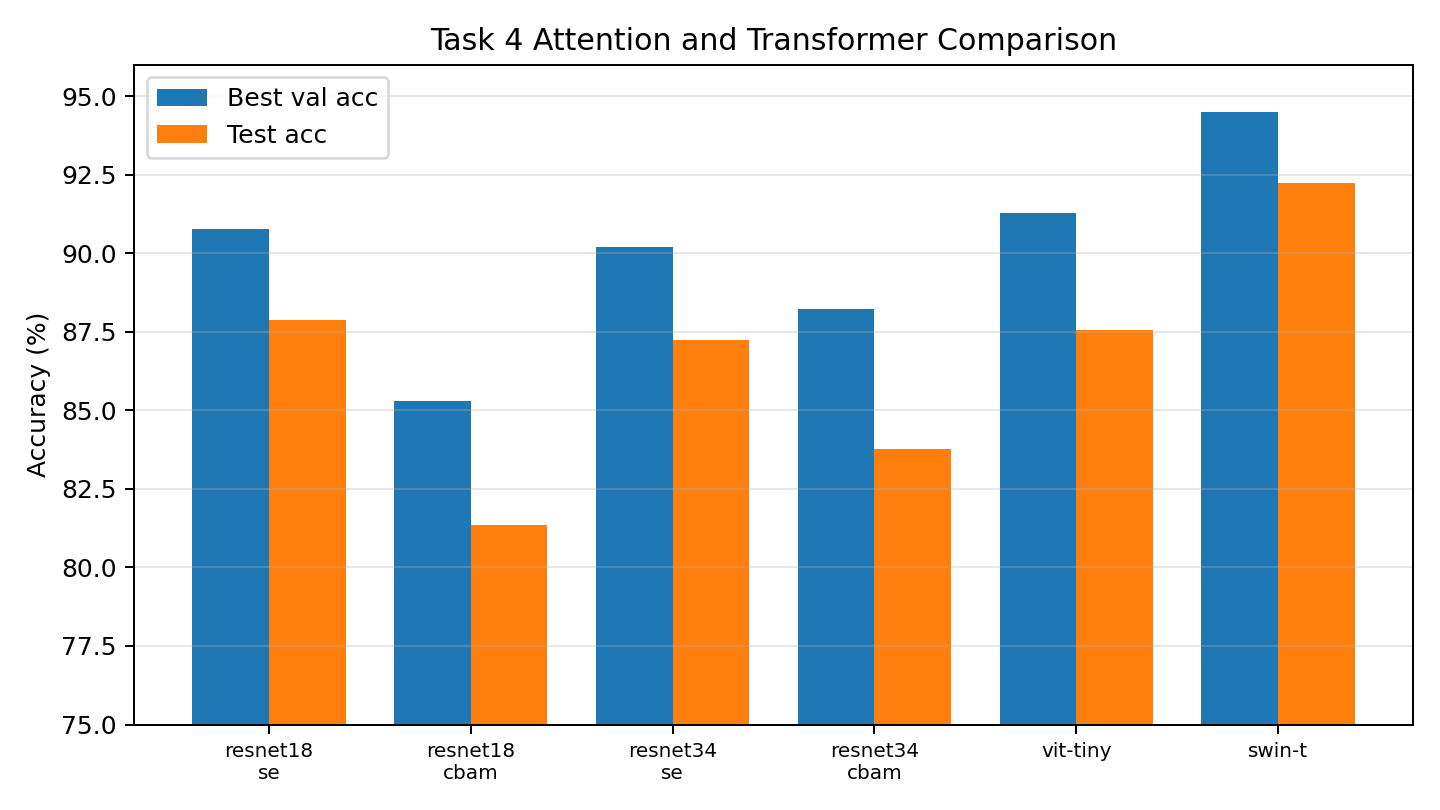
\includegraphics[width=\linewidth]{figures/task4_attention_transformer_comparison.png}
  \caption{Task 4 comparison of attention ResNets and Transformer models. Swin-T is the strongest model in this experiment.}
  \label{fig:task4_compare}
\end{figure}

SE is more stable than CBAM in both depths, but still lower than the plain baselines. A likely reason is that the newly inserted attention layers are randomly initialized, and the small training split may not be enough to tune them well without additional hyperparameter search. Figure~\ref{fig:task4_compare} shows the same conclusion visually. The SE-ResNet-18 curve in Figure~\ref{fig:task4_se} shows successful training, but its final generalization is still weaker than the plain ResNet-18 run.
% 中文注释：这里解释注意力模块没有提升的可能原因，并强调这不是对方法本身的绝对否定。

\begin{figure}[t]
  \centering
  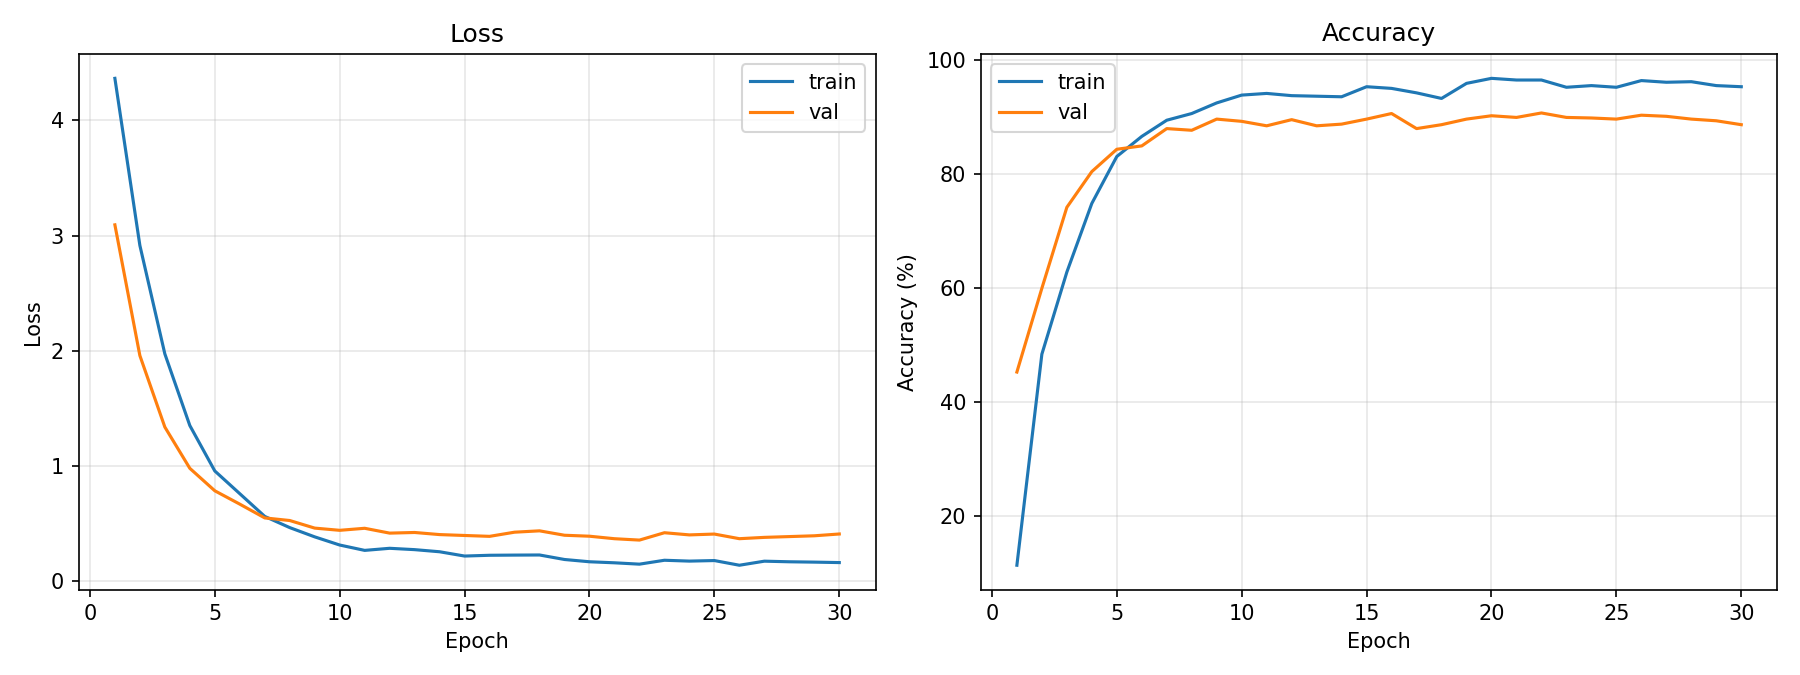
\includegraphics[width=\linewidth]{figures/task4_resnet18_se_curve.png}
  \caption{Task 4 SE-ResNet-18 training and validation curves.}
  \label{fig:task4_se}
\end{figure}

For Transformer models, ViT-Tiny reaches 87.58\% test accuracy, which is lower than the ResNet baselines. Swin-T reaches 94.51\% best validation accuracy and 92.24\% test accuracy, making it the best overall model in my experiments. I do not interpret the ViT-Tiny result as evidence that ViT is generally worse; it may need a more suitable fine-tuning recipe. However, the Swin-T result shows that a pretrained hierarchical Transformer can be very competitive on Flowers102.
% 中文注释：这里说明 Swin-T 是整体最佳模型，而 ViT-Tiny 表现较低需要谨慎解释。

\section{Discussion}

Across the four tasks, ImageNet pretraining is the strongest and most reliable factor. The scratch models perform poorly because the Flowers102 training set contains only 1020 images, so random initialization has too little supervision to learn robust visual representations. Hyperparameter tuning also matters: the best ResNet runs use a slightly smaller classifier learning rate than the baseline. Training longer does not automatically improve test accuracy, which suggests that overfitting and checkpoint selection are important.
% 中文注释：讨论部分总结预训练、小样本、学习率和训练轮数之间的关系。

The comparison between ResNet-18 and ResNet-34 is not one-sided. ResNet-18 is slightly better in the baseline, while ResNet-34 becomes better after learning-rate tuning. Attention modules are not stable improvements here, and CBAM hurts more than SE. Among all models, Swin-T gives the highest test accuracy, but this conclusion is based on the tested hyperparameters only.
% 中文注释：这里总结模型深度、注意力模块和 Transformer 对比的主要发现。

\section{Conclusion}

The best overall model is Swin-T with 92.24\% test accuracy. The best ResNet-only model is ResNet-34 with classifier learning rate $5\times10^{-4}$, backbone learning rate $5\times10^{-5}$, batch size 32, and 30 epochs, reaching 91.59\% test accuracy. ImageNet pretraining is essential: it improves ResNet-18 by 61.44 percentage points and ResNet-34 by 68.63 percentage points over scratch training. The main limitation is that the experiments use a limited hyperparameter grid and were run on local Mac hardware, so future work should include repeated seeds, learning-rate schedules, and more architecture-specific tuning.
% 中文注释：结论总结最佳模型、最佳 ResNet 配置、预训练收益和实验不足。

\appendix

\section{Complete Results}

Table~\ref{tab:appendix_all} lists all experiment folders used in this report.
% 中文注释：附录列出完整实验结果，便于检查每个实验目录对应的数值。

\begin{table}[h]
  \caption{Complete experiment summary.}
  \label{tab:appendix_all}
  \centering
  \tiny
  \resizebox{\linewidth}{!}{%
\begin{tabular}{llllrrrrrrrl}
\toprule
Task & Model & Attn & Init & Epochs & BS & BB LR & Cls LR & LR & Best Val & Test & Folder \\
\midrule
task1\_baseline & resnet18 & none & pretrained & 30 & 32 & 1e-4 & 1e-3 & -- & 92.16 & 89.85 & task1\_resnet18 \\
task1\_baseline & resnet34 & none & pretrained & 30 & 32 & 1e-4 & 1e-3 & -- & 91.76 & 89.64 & task1\_resnet34 \\
task2\_hparam & resnet18 & none & pretrained & 10 & 32 & 1e-4 & 1e-3 & -- & 91.18 & 89.19 & task2\_resnet18\_epoch10\_blr1e-4\_clr1e-3\_bs32 \\
task2\_hparam & resnet18 & none & pretrained & 30 & 16 & 1e-4 & 1e-3 & -- & 91.76 & 87.40 & task2\_resnet18\_epoch30\_blr1e-4\_clr1e-3\_bs16 \\
task2\_hparam & resnet18 & none & pretrained & 30 & 32 & 1e-5 & 1e-4 & -- & 89.22 & 85.59 & task2\_resnet18\_epoch30\_blr1e-5\_clr1e-4\_bs32 \\
task2\_hparam & resnet18 & none & pretrained & 30 & 32 & 5e-5 & 5e-4 & -- & 94.12 & 90.62 & task2\_resnet18\_epoch30\_blr5e-5\_clr5e-4\_bs32 \\
task2\_hparam & resnet18 & none & pretrained & 30 & 32 & 1e-4 & 1e-3 & -- & 92.16 & 89.85 & task2\_resnet18\_epoch30\_blr1e-4\_clr1e-3\_bs32 \\
task2\_hparam & resnet18 & none & pretrained & 30 & 32 & 2e-4 & 2e-3 & -- & 89.31 & 85.64 & task2\_resnet18\_epoch30\_blr2e-4\_clr2e-3\_bs32 \\
task2\_hparam & resnet18 & none & pretrained & 50 & 32 & 1e-4 & 1e-3 & -- & 92.25 & 89.74 & task2\_resnet18\_epoch50\_blr1e-4\_clr1e-3\_bs32 \\
task2\_hparam & resnet34 & none & pretrained & 10 & 32 & 1e-4 & 1e-3 & -- & 91.76 & 89.64 & task2\_resnet34\_epoch10\_blr1e-4\_clr1e-3\_bs32 \\
task2\_hparam & resnet34 & none & pretrained & 30 & 16 & 1e-4 & 1e-3 & -- & 91.18 & 88.78 & task2\_resnet34\_epoch30\_blr1e-4\_clr1e-3\_bs16 \\
task2\_hparam & resnet34 & none & pretrained & 30 & 32 & 1e-5 & 1e-4 & -- & 90.98 & 88.06 & task2\_resnet34\_epoch30\_blr1e-5\_clr1e-4\_bs32 \\
task2\_hparam & resnet34 & none & pretrained & 30 & 32 & 5e-5 & 5e-4 & -- & 93.53 & 91.59 & task2\_resnet34\_epoch30\_blr5e-5\_clr5e-4\_bs32 \\
task2\_hparam & resnet34 & none & pretrained & 30 & 32 & 1e-4 & 1e-3 & -- & 91.76 & 89.64 & task2\_resnet34\_epoch30\_blr1e-4\_clr1e-3\_bs32 \\
task2\_hparam & resnet34 & none & pretrained & 30 & 32 & 2e-4 & 2e-3 & -- & 87.84 & 85.85 & task2\_resnet34\_epoch30\_blr2e-4\_clr2e-3\_bs32 \\
task2\_hparam & resnet34 & none & pretrained & 50 & 32 & 1e-4 & 1e-3 & -- & 91.76 & 89.64 & task2\_resnet34\_epoch50\_blr1e-4\_clr1e-3\_bs32 \\
task3\_ablation & resnet18 & none & pretrained & 30 & 32 & 1e-4 & 1e-3 & -- & 92.16 & 89.85 & task3\_resnet18\_pretrained \\
task3\_ablation & resnet18 & none & scratch & 30 & 32 & 1e-3 & 1e-3 & -- & 32.16 & 28.41 & task3\_resnet18\_scratch \\
task3\_ablation & resnet34 & none & pretrained & 30 & 32 & 1e-4 & 1e-3 & -- & 91.76 & 89.64 & task3\_resnet34\_pretrained \\
task3\_ablation & resnet34 & none & scratch & 30 & 32 & 1e-3 & 1e-3 & -- & 25.98 & 21.01 & task3\_resnet34\_scratch \\
task4\_attention & resnet18 & cbam & pretrained & 30 & 32 & 1e-4 & 1e-3 & 1e-4 & 85.29 & 81.36 & task4\_resnet18\_cbam \\
task4\_attention & resnet18 & se & pretrained & 30 & 32 & 1e-4 & 1e-3 & 1e-4 & 90.78 & 87.87 & task4\_resnet18\_se \\
task4\_attention & resnet34 & cbam & pretrained & 30 & 32 & 1e-4 & 1e-3 & 1e-4 & 88.24 & 83.77 & task4\_resnet34\_cbam \\
task4\_attention & resnet34 & se & pretrained & 30 & 32 & 1e-4 & 1e-3 & 1e-4 & 90.20 & 87.23 & task4\_resnet34\_se \\
task4\_attention & vit\_tiny & none & pretrained & 30 & 8 & 1e-4 & 1e-3 & 1e-4 & 91.27 & 87.58 & task4\_vit\_tiny \\
task4\_attention & swin\_t & none & pretrained & 30 & 32 & 1e-4 & 1e-3 & 1e-4 & 94.51 & 92.24 & task4\_swin\_t \\
\bottomrule
\end{tabular}
}%

\end{table}

\section{Representative Commands}

\begin{verbatim}
python scripts/prepare_data.py --data_dir ./data
python scripts/train_task1_baseline.py --model resnet18 --data_dir ./data \
  --epochs 30 --batch_size 32 --backbone_lr 1e-4 --classifier_lr 1e-3 \
  --weight_decay 1e-4 --optimizer adamw --num_workers 0 --device mps
python scripts/train_task4_attention.py --model swin_t --pretrained true \
  --data_dir ./data --epochs 30 --batch_size 32 --lr 1e-4 \
  --weight_decay 1e-4 --optimizer adamw --num_workers 0 --device mps
\end{verbatim}

\bibliographystyle{plainnat}
\bibliography{references}

\end{document}
